\chapter{Программная среда комплекс моделирования нелинейных динамических систем ``qontrol''}
\label{chapter_qontrol}

\section{Анализ существующих систем} %  % {{{1 ---------------------------------------------

\paragraph{Matlab, simulink}

Этот коммерческий продукт является стандартом де-факто
в исследовательских работах в задачах моделирования динамических систем,
а также многих других областях. Среди положительных особенностей следует
отметить наличие большого количества пакетов для решения разнообразных задач,
развитый, хоть и немного ограниченный язык программирования, поддержка множества
вычислительных платформ. Из недостатков следует отметить заметное навязывание
исследователю методов и приёмов работы, сокрытие от пользователя деталей применяемых
алгоритмов, непомерную стоимость, ограниченные возможности работы с оборудованием.


\paragraph{Scilab, octave}

Являются Open-source аналогами Matlab, имеют практически совместимый язык программирования,
набор базовых возможностей и пакетов. Отличаются заметно меньшим количеством доступных
пакетов, что достаточно хорошо перекрывается открытостью платформы, что позволяет
с меньшими усилиями реализовывать свои расширения. Бесплатность, открытость
и свободная лицензия (CeCILL, GPLv3+) представляют серьёзные преимущества для
исследователя. Тем не менее, совместимость с Matlab имеет и обратную сторону,
а именно ограниченность языка и навязывание приёмов работы.

\paragraph{Multisim}

Специальный коммерческий продукт, предназначенный для моделирования, проектирования
и анализа преимущественно электронных схем. Благодаря большой базе электронных
компонентов и применению специальных алгоритмов заметно упрощает
разработку и моделирование именно электронных устройств. Наличие
набора ``идеальных'' элементов, применяемых в теории управления,
позволяет в какой-то мере расширить круг задач за пределы
электронного моделирования. Тем не менее, этот продукт остаётся
узкоспециализированным средством. Более того, закрытость и ограниченность средств настройки
применяемых алгоритмов моделирования не даёт в отдельных случаях
ни получить адекватный результат, ни определить точно причину подобного поведения.

\paragraph{LabView}

Еще один коммерческий продукт, применяемый преимущественно для
моделирования и анализа электронных схем. Отличительной особенностью
данного продукта являются развитые средства взаимодействия
с реальными измерительным приборами исполнительными механизмами.
При этом, список таких внешних устройств определяется
ограниченным набором производителей, и применение собственных
разработок в этом пакете возможно, если создаваемое устройство
симулирует одно из стандартных. Это существенно снижает применимость
данного пакета при взаимодействии с нестандартным оборудованием.



\paragraph{Выводы}

Таким образом, для проведения исследований, связанных с решением
поставленных проблем, требуется разработка как специального программного
обеспечения, так и взаимодействующих с ним аппаратных измерительных средств.



% }}}1

% \section{Требования к системе моделирования} %  % {{{1 ---------------------------------------------
%
% Созданный ?


% }}}1


\section{Основы построения программной среды} %  % {{{1 ------------------------------

Для разработки комплекса в качестве базового языка был выбран C++,
как обеспечивающий совмещение гибкости и возможностей разработки
с необходимой скоростью вычислений. Также, данный язык
является полностью применимым для программирования микроконтроллеров
класса STM32, входящих в состав аппаратной части комплекса.

Тем не менее, для реализации возможностей автоматизации
внутри самой программы требуется применение языка,
не требующего предварительной компиляции, достаточно распространённого,
быстрого, поддерживающего объектную модель.
В качестве такого языка был выбран ECMAScript, известный также
как Javascript.

\subsection{Реализация интроспекции}  % {{{2

Для реализации задач гибкого подхода к моделированию, автоматизации
и автоматического построения интерфейсных элементов
требуется получение информации об объектах системы моделирования
в процессе работы программы (интроспекции).
В самом языке C++ в данный момент не средств реализации интроспекции.
Библиотека Qt, используемая в разработке, предоставляет
базовые возможности интроспекции, за счёт использования метакомпилятора ``moc''.

% }}}2


\subsection{Базовые объекты системы и структурная схема модели}  % {{{2


% }}}2




% }}}1

\section{Пользовательский интерфейс комплекса} %  % {{{1 ----------------------------------------

Пользовательский интерфейс программы ``qontrol'' был создан с помощью
средств, предоставляемых библиотекой Qt.

\begin{figure}[htb!]
  \begin{center}
    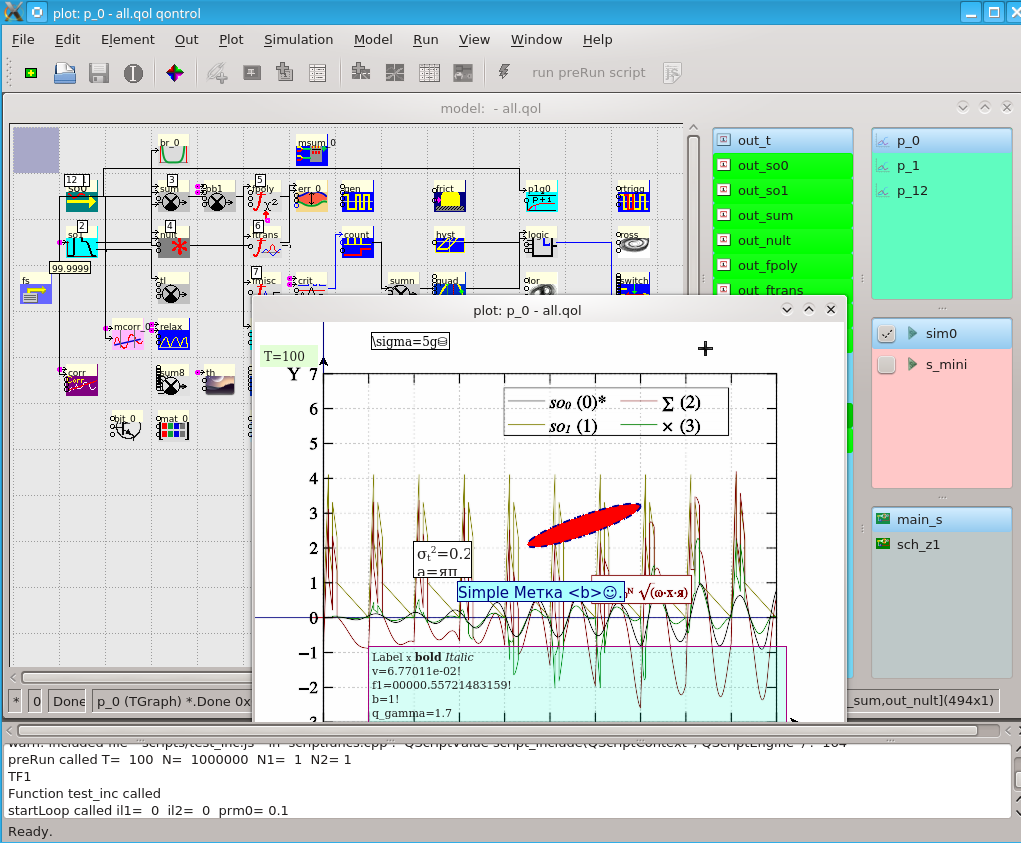
\includegraphics[width=0.96\textwidth]{p/qontrol_all.png}
  \end{center}
  \caption{Общий вид интерфейса пользователя программы ``qontrol''}
  \label{atu:f:qontrol_all}
\end{figure}



\begin{figure}[htb!]
  \begin{center}
    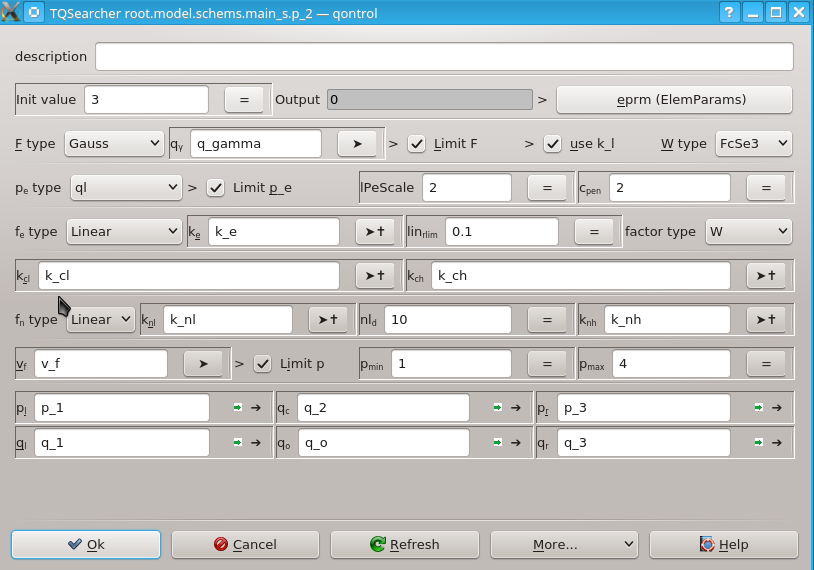
\includegraphics[width=0.7\textwidth]{p/qontrol_tqsearch.png}
  \end{center}
  \caption{Диалоговое окно с элементами интерфейса, автоматически созданными для объекта ``TQSearcher''}
  \label{atu:f:qontrol_qsearch}
\end{figure}



\begin{figure}[htb!]
  \begin{center}
    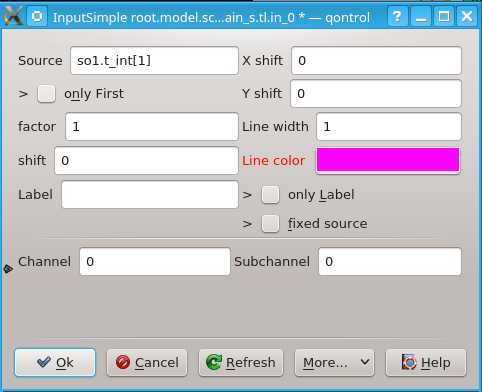
\includegraphics[width=0.5\textwidth]{p/qontrol_link.png}
  \end{center}
  \caption{Диалоговое окно, которое позволяет задать параметры связи между объектами}
  \label{atu:f:qontrol_link}
\end{figure}


\begin{figure}[htb!]
  \begin{center}
    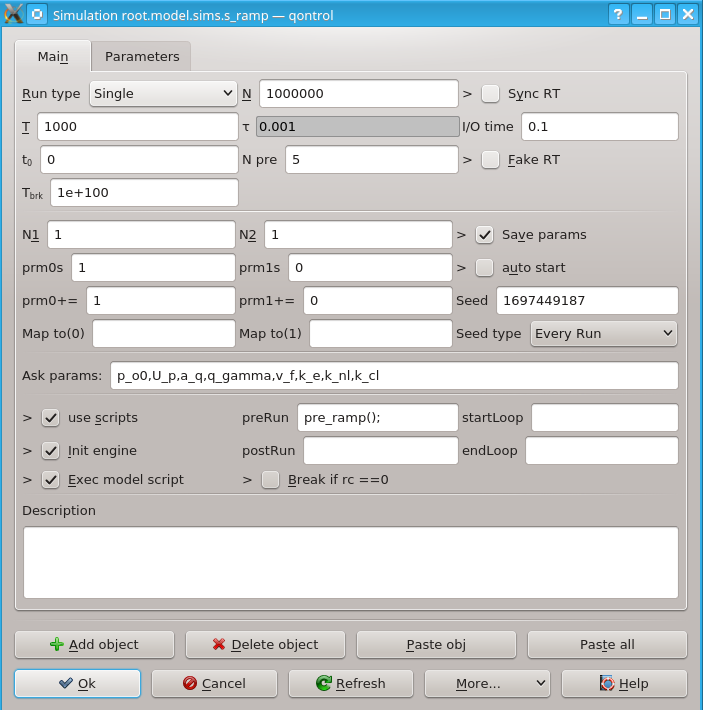
\includegraphics[width=0.7\textwidth]{p/qontrol_task.png}
  \end{center}
  \caption{Диалоговое окно, предназначенное для задания параметров моделирования}
  \label{atu:f:qontrol_simul}
\end{figure}


\begin{figure}[htb!]
  \begin{center}
    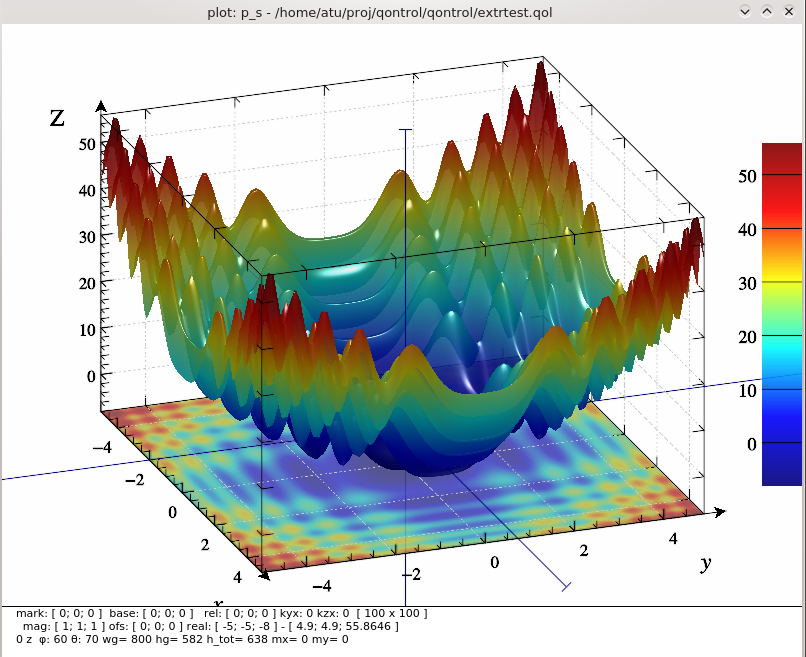
\includegraphics[width=0.7\textwidth]{p/qontrol_3d_a.png}
  \end{center}
  \caption{Окно,предназначенное для отображения графиков}
  \label{atu:f:qontrol_3d}
\end{figure}
% }}}1

\section{Основные подходы к } %  {{{1 --------------------------------------------- 

% }}}1

\section{Выводы по разделу \thechapter} %  % {{{1 ---------------------------------------------

Создана программная среда ``qontrol'', предназначенная для моделирования
нелинейных динамических систем, обладающая набором качеств,
которые существенно упрощают процесс моделирования,
создания новых систем идентификации и управления.
К характеристикам программы следует отнести:

\begin{itemize}

  \item
    Универсальность, позволяющая создавать модели сложных динамических систем,
    с возможностью комбинирования и группировки элементов системы.

  \item
    Развитые средства обработки и представления данных.

  \item
    Удобный интерфейс пользователя.

  \item
    Высокая скорость моделирования.

  \item
    Возможность запускать программу в консольном режиме, без графического интерфейса
    для проведения моделирования в пакетном режиме.

  \item
    Автоматическое построение интерфейса пользователя на основе
    данных, представляемых моделируемым элементом.

  \item
    Возможность реализации сложных задач моделирования, которые не вписываются
    в набор базовых действий, за счёт применения встроенного языка программирования,
    основанного на JavaScript, и возможностью доступа к функциям программной среды.

  \item
    Широкие возможности по отображение информации в графическом виде.

  \item
    Возможность взаимодействия с другими программными и аппаратно-программными
    комплексами.


  \item
    Открытый исходный код, что даёт возможность как применять элементы созданной
    программы в своих разработках, так и дополнять программу своими элементами.


  \item
    Open-source лицензия и свободное распространение,
    что позволяет без существенных затрат использовать программную среду
    при проведении исследований и в учебном процессе.

\end{itemize}


% }}}1


% vim: fdm=marker ft=tex
